% /*
%  * ----------------------------------------------------------------------------
%  * "THE BEER-WARE LICENSE" (Revision 42):
%  * <michi.wieland@hotmail.com> wrote this file. As long as you retain this notice you
%  * can do whatever you want with this stuff. If we meet some day, and you think
%  * this stuff is worth it, you can buy me a beer in return. Michael Wieland
%  * ----------------------------------------------------------------------------
%  */

\documentclass[
a4paper,
oneside,
10pt,
fleqn,
headsepline,
toc=listofnumbered, 
bibliography=totocnumbered]{scrartcl}

% deutsche Trennmuster etc.
\usepackage[T1]{fontenc}
\usepackage[utf8]{inputenc}
\usepackage[english, ngerman]{babel} % \selectlanguage{english} if  needed
\usepackage{lmodern} % use modern latin fonts

% Custom commands
\newcommand{\AUTHOR}{Michael Wieland}
\newcommand{\INSTITUTE}{Hochschule für Technik Rapperswil}
\newcommand{\GITHUB}{https://github.com/michiwieland/hsr-zusammenfassungen}
\newcommand{\LICENSEURL}{https://en.wikipedia.org/wiki/Beerware}
\newcommand{\LICENSE}{
"THE BEER-WARE LICENSE" (Revision 42):
<michi.wieland@hotmail.com> wrote this file. As long as you retain this notice you
can do whatever you want with this stuff. If we meet some day, and you think
this stuff is worth it, you can buy me a beer in return. Michael Wieland	
}

% Jede Überschrift 1 auf neuer Seite
\let\stdsection\section
\renewcommand\section{\clearpage\stdsection}

% Multiple Authors
\usepackage{authblk}

% Include external pdf
\usepackage{pdfpages}

% Layout / Seitenränder
\usepackage{geometry}

% Inhaltsverzeichnis
\usepackage{makeidx} 
\makeindex

\usepackage{url}
\usepackage[pdfborder={0 0 0}]{hyperref}
\usepackage[all]{hypcap}
\usepackage{hyperxmp} % for license metadata

% Glossar und Abkürzungsverzeichnis
\usepackage[acronym,toc,nopostdot]{glossaries}
\glossarystyle{altlist}
\usepackage{xparse}
\DeclareDocumentCommand{\newdualentry}{ O{} O{} m m m m } {
	\newglossaryentry{gls-#3}{
		name={#4 : #5},
		text={#5\glsadd{#3}},
		description={#6},
		#1
	}
	\makeglossaries
	\newacronym[see={[Siehe:]{gls-#3}},#2]{#3}{#4}{#5\glsadd{gls-#3}}
}
\makeglossaries

% Mathematik
\usepackage{amsmath}
\usepackage{amssymb}
\usepackage{amsfonts}
\usepackage{enumitem}

% Images
\usepackage{graphicx}
\graphicspath{{images/}} % default paths

% Boxes
\usepackage{fancybox}

%Tables
\usepackage{tabu}
\usepackage{booktabs} % toprule, midrule, bottomrule
\usepackage{array} % for matrix tables

% Multi Columns
\usepackage{multicol}

% Header and footer
\usepackage{scrlayer-scrpage}
\setkomafont{pagehead}{\normalfont}
\setkomafont{pagefoot}{\normalfont}
\automark*{section}
\clearpairofpagestyles
\ihead{\headmark}
\ohead{\AUTHOR}
\cfoot{\pagemark}

% Pseudocode
\usepackage{algorithmic}
\usepackage[linesnumbered,ruled]{algorithm2e}

% Code Listings
\usepackage{listings}
\usepackage{color}
\usepackage{beramono}

\definecolor{bluekeywords}{rgb}{0,0,1}
\definecolor{greencomments}{rgb}{0,0.5,0}
\definecolor{redstrings}{rgb}{0.64,0.08,0.08}
\definecolor{xmlcomments}{rgb}{0.5,0.5,0.5}
\definecolor{types}{rgb}{0.17,0.57,0.68}

\lstdefinestyle{visual-studio-style}{
	language=[Sharp]C,
	columns=flexible,
	showstringspaces=false,
	basicstyle=\footnotesize\ttfamily, 
	commentstyle=\color{greencomments},
	morekeywords={partial, var, value, get, set},
	keywordstyle=\bfseries\color{bluekeywords},
	stringstyle=\color{redstrings},
	breaklines=true,
	breakatwhitespace=true,
	tabsize=4,
	numbers=left,
	numberstyle=\tiny\color{black},
	frame=lines,
	showspaces=false,
	showtabs=false,
	escapeinside={£}{£},
}

\definecolor{DarkPurple}{rgb}{0.4, 0.1, 0.4}
\definecolor{DarkCyan}{rgb}{0.0, 0.5, 0.4}
\definecolor{LightLime}{rgb}{0.3, 0.5, 0.4}
\definecolor{Blue}{rgb}{0.0, 0.0, 1.0}

\lstdefinestyle{cevelop-style}{
	language=C++,  
	columns=flexible,
	showstringspaces=false,     
	basicstyle=\footnotesize\ttfamily, 
	keywordstyle=\bfseries\color{DarkPurple},
	commentstyle=\color{LightLime},
	stringstyle=\color{Blue}, 
	escapeinside={£}{£}, % latex scope within code      
	breaklines=true,
	breakatwhitespace=true,
	showspaces=false,
	showtabs=false,
	tabsize=4,
	morekeywords={include,ifndef,define},
	numbers=left,
	numberstyle=\tiny\color{black},
	frame=lines,
}

\lstdefinestyle{eclipse-style}{
	language=Java,  
	columns=flexible,
	showstringspaces=false,     
	basicstyle=\footnotesize\ttfamily, 
	keywordstyle=\bfseries\color{DarkPurple},
	commentstyle=\color{LightLime},
	stringstyle=\color{Blue}, 
	escapeinside={£}{£}, % latex scope within code      
	breaklines=true,
	breakatwhitespace=true,
	showspaces=false,
	showtabs=false,
	tabsize=4,
	morekeywords={length},
	numbers=left,
	numberstyle=\tiny\color{black},
	frame=lines,
}
\lstset{style=eclipse-style}



% Theorems \begin{mytheo}{title}{label}
\usepackage{tcolorbox}
\tcbuselibrary{theorems}
\newtcbtheorem[number within=section]{definiton}{Definition}%
{fonttitle=\bfseries}{def}
\newtcbtheorem[number within=section]{remember}{Merke}%
{fonttitle=\bfseries}{rem}
\newtcbtheorem[number within=section]{hint}{Hinweis}%
{fonttitle=\bfseries}{hnt}

% Dokumentinformationen
\newcommand{\SUBJECT}{Zusammenfassung}
\newcommand{\TITLE}{Analysis für Informatiker 2}

% pdf metadata
\hypersetup{
	pdfauthor={\AUTHOR},
	pdftitle={\SUBJECT \TITLE},
	pdfcopyright={\LICENSE},
	pdflicenseurl={\LICENSEURL}
}

\begin{document}
	
% Front page
\title{\TITLE}
\subject{\SUBJECT}
\author{\AUTHOR}
\affil{\INSTITUTE}
\date{\today}
\maketitle

\vfill

% Participate
\paragraph{Mitmachen} \hfill \\
Falls Du an diesem Dokument mitarbeiten willst, kannst Du das Dokument
auf GitHub unter \url{\GITHUB} forken.

% Licence
\paragraph{Lizenz} \hfill \\
\LICENSE

% Table of contents
\tableofcontents


% Glossar and acronyms (if included \loadglsentries{glossar})
\printglossary[type=\acronymtype]
\printglossary
\glsaddall


\section{Grundlagen}
\subsection{Plots}
\begin{figure}[h]
	\centering
	\begin{minipage}[t]{0.4\textwidth}
		\centering
		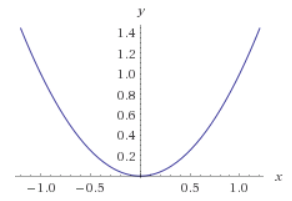
\includegraphics[width=\textwidth]{images/graph_x_2}
		\caption{$x^2$}
	\end{minipage}
	\begin{minipage}[t]{0.4\textwidth}
		\centering
		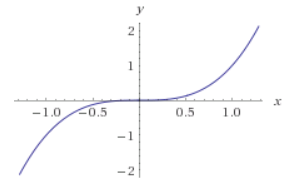
\includegraphics[width=\textwidth]{images/graph_x_3}
		\caption{$x^3$}
 	\end{minipage}
\end{figure}
\begin{figure}[ht!]
	\centering
	\begin{minipage}[t]{0.4\textwidth}
		\centering
		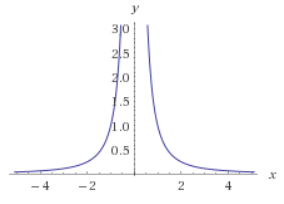
\includegraphics[width=\textwidth]{images/graph_x_-2}
		\caption{$x^{-2}$}
	\end{minipage}
	\begin{minipage}[t]{0.4\textwidth}
		\centering
		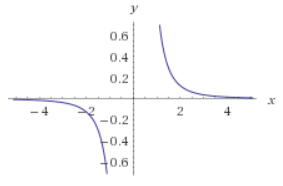
\includegraphics[width=\textwidth]{images/graph_x_-3}
		\caption{$x^{-3}$}
	\end{minipage}
\end{figure}
\begin{figure}[ht!]
	\centering
	\begin{minipage}[t]{0.4\textwidth}
		\centering
		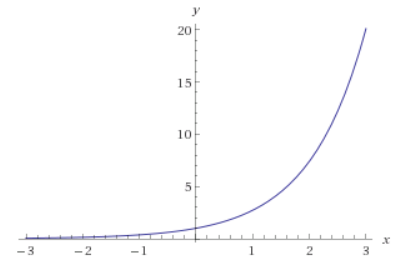
\includegraphics[width=\textwidth]{images/graph_e_x}
		\caption{$e^{x}$}
		\begin{itemize}
			\item Basis muss grösser 0 sein
			\item Exponenten $\in \mathbb{R}$
			\item Gibt immer Werte grösser 0 zurück
			\item Schneidet bei $x=0$ die Y-Achse (Ordinate) $\Rightarrow e^0 = 1$
		\end{itemize}
	\end{minipage}
	\begin{minipage}[t]{0.4\textwidth}
		\centering
		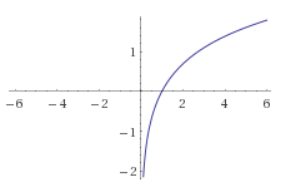
\includegraphics[width=\textwidth]{images/graph_ln_x}
		\caption{$ln(x)$}
		\begin{itemize}
			\item Nimmt nur $\mathbb{R}^{+} \ 0$ entgegen
			\item Liefert $\mathbb{R}$ zurück 
			\item $ln(0)$ ist nicht definiert ($-\infty$)
			\item Hat bei $ln(1)$ denn Nulldurchgang
		\end{itemize}
	\end{minipage}
\end{figure}
\begin{figure}[ht!]
	\centering
	\begin{minipage}[t]{0.4\textwidth}
		\centering
		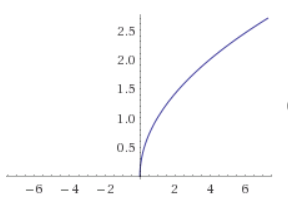
\includegraphics[width=\textwidth]{images/graph_sqrt_x}
		\caption{$\sqrt{x}$}
		\begin{itemize}
			\item Nimmt nur $\mathbb{R^{+}}$ entgegen
		\end{itemize}
	\end{minipage}
	\begin{minipage}[t]{0.4\textwidth}
		\centering
		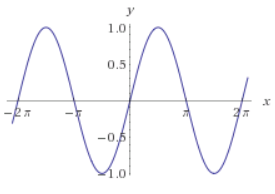
\includegraphics[width=\textwidth]{images/graph_sin_x}
		\caption{$sin(x)$}
		\begin{itemize}
			\item Nimmt $\mathbb{R}$ entgegen
			\item Gibt Werte im Intervall $\left[-1;1\right]$ zurück
			\item Nur eingeschränkt umkehrbar $\Rightarrow sin(x)_{[-\frac{\pi}{2};\frac{\pi}{2}]}$
		\end{itemize}
	\end{minipage}
\end{figure}
\begin{figure}[ht!]
	\centering
	\begin{minipage}[t]{0.4\textwidth}
		\centering
		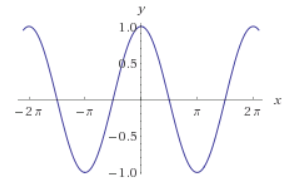
\includegraphics[width=\textwidth]{images/graph_cos_x}
		\caption{$cos(x)$}
		\begin{itemize}
			\item Nimmt $\mathbb{R}$ entgegen
			\item Gibt Werte im Intervall $\left[-1;1\right]$ zurück
			\item Nur eingeschränkt umkehrbar $\Rightarrow cos(x)_{[0;\pi]}$
		\end{itemize}
	\end{minipage}
	\begin{minipage}[t]{0.4\textwidth}
		\centering
		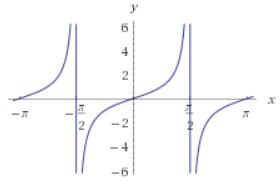
\includegraphics[width=\textwidth]{images/graph_tan_x}
		\caption{$tan(x)$}
		\begin{itemize}
			\item Kreutzt bei Vielfachen von $\pi$ die X-Achse (Abszisse)
			\item $x \in \mathbb{R} | x \neq \frac{\pi}{2} + k \cdot \pi$
			\item Nur eingeschränkt umkehrbar $\Rightarrow tan(x)_{(-\frac{\pi}{2};\frac{\pi}{2})}$
		\end{itemize}
	\end{minipage}
\end{figure}
\begin{figure}[ht!]
	\centering
	\begin{minipage}[t]{0.4\textwidth}
		\centering
		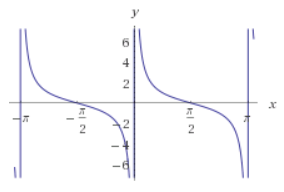
\includegraphics[width=\textwidth]{images/graph_cot_x}
		\caption{$cot(x)$}
	\end{minipage}
	\begin{minipage}[t]{0.4\textwidth}
		\centering
		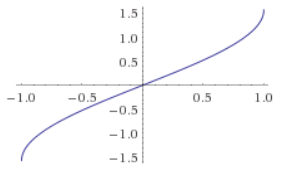
\includegraphics[width=\textwidth]{images/graph_arcsin_x}
		\caption{$arcsin(x)$}
		\begin{itemize}
			\item $y \in [-\frac{\pi}{2};\frac{\pi}{2}]$
		\end{itemize}
	\end{minipage}
\end{figure}
\begin{figure}[ht!]
	\centering
	\begin{minipage}[t]{0.4\textwidth}
		\centering
		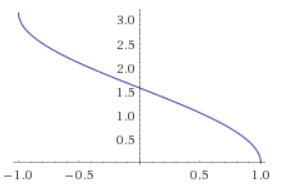
\includegraphics[width=\textwidth]{images/graph_arccos_x}
		\caption{$arccos(x)$}
		\begin{itemize}
			\item $ y \in [0;\pi]$
		\end{itemize}
	\end{minipage}
	\begin{minipage}[t]{0.4\textwidth}
		\centering
		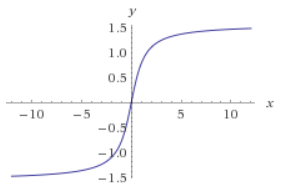
\includegraphics[width=\textwidth]{images/graph_arctan_x}
		\caption{$arctan(x)$}
		\begin{itemize}
			\item $y \in  (-\frac{\pi}{2};\frac{\pi}{2})$
		\end{itemize}
	\end{minipage}
\end{figure}
\begin{figure}[ht!]
	\centering
	\begin{minipage}[t]{0.4\textwidth}
		\centering
		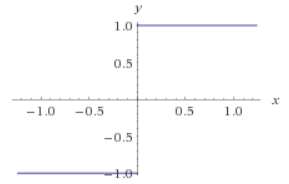
\includegraphics[width=\textwidth]{images/graph_signum}
		\caption{$signum(x)$}
	\end{minipage}
\end{figure}

\clearpage

\subsection{Verschiebungen von Graphen}
\subsubsection{Spieglungen}
\begin{description}
	\item[An X-Achse] $f(x) \Rightarrow -f(x)$
	\item[An Y-Achse] $f(x) \Rightarrow f(-x)$
	\item[Am Nullpunkt] $f(x) \Rightarrow -f(-x)$
\end{description}

\subsubsection{Entlang der X-Achse}
\begin{description}
	\item[Verschiebung nach rechts] $f(x) \Rightarrow f(x - k)$
	\item[Verschiebung nach links] $f(x) \Rightarrow f(x + k)$
	\item[Strecken] $f(x) \Rightarrow f(\frac{x}{k})$
	\item[Stauchen] $f(x) \Rightarrow f(kx)$
\end{description}

\subsubsection{Entlang der Y-Achse}
\begin{description}
	\item[Verschiebung nach oben] $f(x) \Rightarrow f(x) + k$
	\item[Verschiebung nach unten] $f(x) \Rightarrow f(x) - k$
	\item[Strecken] $f(x) \Rightarrow k \cdot f(x)$
	\item[Stauchen] $f(x) \Rightarrow \frac{1}{k} \cdot f(x)$
\end{description}

\subsection{Ableitungsregeln}
\begin{tabu} to \linewidth {|X|X|}
	\hline
	Funktion 	& Ableitung \\ 
	\hline\hline
	$x^a$ & $a \cdot x^{a-1}$ \\ \hline
	1 & 0 \\ \hline
	$x$ & 1 \\ \hline
	$x^2$ & $2x$ \\ \hline
	$\frac{1}{x}$ & $-\frac{1}{x^2}$ \\ \hline
	$\sqrt{x}$ & $\frac{1}{2 \cdot \sqrt{x}}$ \\ \hline
	$e^x$ & $e^x$ \\ \hline
	$a^x$ & $ln(a) \cdot a^x$  \\ \hline
	$ln(x)$ & $\frac{1}{x}$ \\ \hline
	$log_b(x)$ & $\frac{1}{ln(b) \cdot x}$ \\ \hline
	$sin(x)$ & $cos(x)$ \\ \hline
	$cos(x)$ & $-sin(x)$ \\ \hline
	$tan(x)$ & $\frac{1}{cos^2(x)}$ \\ \hline
	$tan(x)$ & $1 + tan^2(x)$ \\ \hline
	$arcsin(x)$ & $\frac{1}{\sqrt{1-x^2}}$ \\ \hline
	$arccos(x)$ & $-\frac{1}{\sqrt{1-x^2}}$ \\ \hline
	$arctan(x)$ & $\frac{1}{1+x^2}$ \\ \hline
\end{tabu}

\subsection{Stammfunktion}
\begin{tabu} to \linewidth {|X|X|X|}
	\hline
	Funktion 	& Stammfunktion & Bemerkung \\ 
	\hline\hline
	$x^a$ & $\frac{1}{a+1}x^{a+1} + const$ & \\ \hline
	$x^a$ & $ln(|x|) + const$ & Falls $a=-1$ \\ \hline
	1 & $x + const$ & \\ \hline
	$x$ & $\frac{1}{2}x^2 + const$ & \\ \hline
	$x^2$ & $\frac{1}{3}x^3 + const$ & \\ \hline
	$\frac{1}{x}$ & $ln(|x|) + const$ & \\ \hline
	$\sqrt{x}$ & $\frac{2}{3}x^{\frac{3}{2}}+const$ & \\ \hline
	$e^x$ & $e^x + const$ & \\ \hline
	$sin(x)$ & $-cos(x) + const$ & \\ \hline
	$cos(x)$ & $sin(x) + const$ & \\ \hline
\end{tabu}

\subsection{Logarithmen}
\[
	log(x \cdot y) = log(x) + log(y)
\]
\[
	log(\frac{x}{y}) = log(x) - log(y)
\]
\[
	log(x^y) = y \cdot log(x)
\]

\subsection{Trigonometrische Funktionen}
\[
	cos(-x) = cos(x)
\]
\[
	sin(-x) = -sin(x)
\]

\subsection{Konstanten}
\begin{align*}
	\sqrt{2} &\approx 1.414 \\
	\sqrt{3} &\approx 1.732 \\
	e &\approx 2.718 \\
	\pi &\approx 3.141
\end{align*}

\subsection{Polynomdivision}
\paragraph{Vorgehen}
\begin{enumerate}
	\item Dividieren des grössten Exponenten durch den x-Term im Divisor
	\item Nun wird das Resultat mit dem kompletten Divisor multipliziert und und das den Divident geschrieben.
	\item Danach zieht man das Resultat aus der Multiplikation vom Divident ab
	\item Zurück zu Schritt 1 mit dem Resultat aus der Subtraktion
\end{enumerate}
\begin{figure}[h]
	\centering
	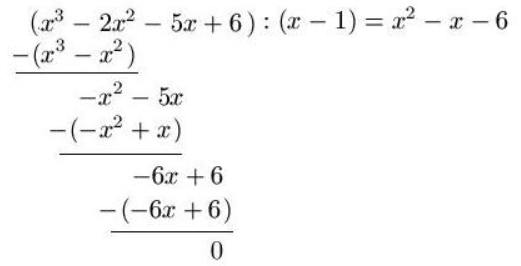
\includegraphics[width=0.3\linewidth]{images/polynomdivision}
	\caption{Polynomdivision}
\end{figure}

 
\section{Taylorreihen}
\subsection{Taylorpolynom}

\begin{itemize}
	\item Jede ableitbare Funktion lässt sich durch Polynome approximieren.  
	\item Endliches Polynom mit Ordnung N
	\item Hat Rechenfehler
	\item Taylor Polynom der ersten Ordnung enspricht der Linearisierung
\end{itemize}

\subsection{Taylorreihe}
\begin{itemize}
	\item Unendliches Polynom 
	\item theoretisch keine Rechenfehler
	\item Stimmt entweder exakt oder überhaupt nicht mit der Ausgangsfunktion überein (Konvergenzradius)
\end{itemize}

\subsubsection{Konvergenzradius}
Der Konvergenzradius ist der Bereich um den Entwicklungspunkt $x_0$, in welchem die Taylorreihe den korrekten Wert der Ausgangsfunktion $f(x)$ liefert. Der Konvergenzradius ist also der Abstand vom Entwicklungspunkt bis zur ersten Definitionslücke.

\subsubsection{Definition:}
Taylorpolynom N-Ordnung 
\begin{align}
\begin{split}
f(x) \approx \sum_{i=0}^{N}\frac{f^{(i)}(x_0)}{i!}(x-x_0)^i \text{ für } x \approx x_0 \\
\end{split}
\end{align}	

\subsubsection{Vorgehen}
\begin{enumerate}
	\item Polynom vom Grad N, N-Mal ableiten
	\item Entwicklungspunkt $x_0$ in alle Ableitungen einsetzen und ausrechnen
	\item Koeffizienten notieren 
	\begin{align*}
	\begin{split}
		K_i = \frac{f^{(i)}(x_0)}{i!} \\
		\begin{aligned}
		\text{mit } \\
		f^{(i)}(x_0) &= \text{Lösung der i-ten Ableitung} \\
		i &= \text{Grad der Ableitung}
		\end{aligned}
	\end{split}
	\end{align*}	
	\item Koeffizienten $K_i$ in Taylorpolynom einfügen
	\begin{align}
	\begin{split}
	f(x) \approx \sum_{i=0}^{n}K_i \cdot (x-x_0)^i \\
	\end{split}
	\end{align}	
	\item Je grösser N gewählt wird, desto besser nähert sich der Entwicklungspunkt $x_0$ dem Resultat x an.
\end{enumerate}

\subsection{Fehlerabschätzung bei Taylorreihen}

\subsection{Definition}
Fehlerabschätzung im Intervall [a;b] für den Fall, dass $x_0 = \frac{a+b}{2}$ und $m \geq |f^{N+1}(x)|$ für alle $x\in [a;b]$
\[
|f(x) - p_{N}(x) | \leq \frac{m(b-a)^{N+1}}{2^{N+1}(N+1)!}
\]

\paragraph{Bemerkung zum Entwicklungspunkt} Der Entwicklungspunkt $x_0$ liegt genau in der Mitte des Intervalls [a;b]

\paragraph{Bemerkung zum Maximum m} \hfill \\
Ein gutes m entspricht dem globalen Maximum der Ableitung $m \geq |f^{N+1}(x)|$. Am besten stellt man sich den Graphen vor und entscheidet dann, ob man $x_0$, $a$ oder $b$ als Funktionsargument $x$ in $f^{N+1}(x)$ nimmt. Oft ist es schwierig m zu bestimmen, weshalb man, wenn a und b nicht alzu weit entfernt sind, einfach den grösseren der beiden Werte als Funktionsargument verwendet:
\[
	m = |f^{N+1}(a)| \lor |f^{N+1}(b)|
\]

\subsection{Beispiel}
Gegeben sei die Tailorreihe der folgenden Funktion um das Entwicklungszentrum $x_0 = 0$
\[
	f(x) = e^{-2x}
\]

So ist das Talorpolynom für das n-te Element 
\begin{align*}
	f^{(n)}(x_0) &= (-2)^n e^{-2x} \\
	f^{(n)}(0) &= (-2)^n
\end{align*}

und die Taylorreihe
\begin{align*}
f(x) &= \sum_{n=0}^{\infty} \frac{(-2)^n}{n!}x^n
\end{align*}

Bestimmen sie den minimalen Grad desjenigen Taylorpolynoms, welches die Funktion $f(x)$ im Intervall $\left[ -\frac{1}{2};\frac{1}{2} \right]$ mit einem Fehler von weniger als $\frac{1}{100}$ berechnen lässt
\begin{enumerate}
	\item m berechnen
	\begin{align*}
		|f^{N+1}(x)| &\leq m \\
		|(-2)^{n+1} e^{-2x}|  &\leq m \\
		2^{n+1} |e^{-2x}|  &\leq m 
	\end{align*}
	\item Globales Maximum für x einsetzen ($a$, $b$ oder $x_0$)
	\begin{align*}
		m &= 2^{n+1} |e^{-2x}| \\
		m &= 2^{n+1} |e^{-2 \cdot -\frac{1}{2}}| \\
		m &= 2^{n+1} |e^{1}|
	\end{align*}
	\item Abschätzen des Rechenfehlers $\Rightarrow$ a,b und m einsetzen und vereinfachen
	\begin{align*}
		|f(x) - p_{N}(x) | &\leq \frac{m(b-a)^{N+1}}{2^{N+1}(N+1)!} \\
		&\leq \frac{2^{N+1} e(\frac{1}{2} + \frac{1}{2})^{N+1}}{2^{N+1}(N+1)!} \\
		&\leq \frac{e}{(N+1)!}
	\end{align*}
	\item Die Zahl N muss nun so gewählt werden dass
	\begin{align*}
	\frac{e}{(N+1)!} &\leq 0.001 \\
	e \cdot 100 &\leq (N+1)!
	\end{align*}
	\item Wertetabelle erstellen mit verschiedenen N der Gleichung \hfill \\
	\begin{tabu} to \linewidth {c l l l l l l}
		\toprule
		N & 0 & 1 & 2 & 3 & 4 & 5\\
		\midrule
		(N+1)! & 1  & 2 & 6 & 24 & 120 & 720 \\
		\bottomrule
	\end{tabu}
	\item Gemäss Tabelle
	\begin{align*}
		e \cdot 100 \approx 270 &\leq 720 \\
		&\Rightarrow \underline{\underline{N \geq5}}
	\end{align*}
	Es ist mindestens ein Taylorpolynom vom Grad 5 nötig
\end{enumerate}


\section{Grenzwerte / Limes}
\subsection{Unendliche Grenzwerte}
Unendliche Grenzwerte sind Grenzwerte der Form $\lim\limits_{x \rightarrow +\infty }f(x)$ rps. $\lim\limits_{x \rightarrow -\infty }f(x)$
\begin{itemize}
	\item Man muss immer Definitionslücken suchen (z.B Teilbar durch 0 möglich?)
	\item Grenzwerte existieren nur wenn die Funktion eine stetige Fortsetzung besitzt.
\end{itemize}

\subsubsection{Vorgehen}
\begin{enumerate}
	\item Bei Brüchen teilt man im Nenner und im Zähler durch den grössten Exponenten. (z.B $x^2$) Eine schnellere Variante ist jedoch, dass man einfach den schnellst wachsenden Exponenten im Zähler und im Nenner herausnimmt und einen neuen Bruch schreibt. (Achtung: Wurzeln etc. bleiben bestehen)
	\[
		\lim\limits_{x \rightarrow \infty} \frac{\sqrt{x^2 - 2x + 1}}{x-1} = \lim\limits_{x \rightarrow \infty} \frac{\sqrt{x^2}}{x} = 1
	\] 
	\item Für jeden einzelnen Term seinen ungefähren Verlauf definieren
	\item Die Grenzwerte zusammen gezählt, ergeben dann den Grenzwert für den ganzen Ausdruck
\end{enumerate}

\paragraph{Beispiele:}
\begin{align*}
	\lim\limits_{x \rightarrow \infty} \frac{3x^2 + 4x - 12}{4 -x^2} &\overset{/x^2}{=} \frac{\frac{1}{x^2} \cdot (3x^2 + 4x -12)}{\frac{1}{x^2} \cdot 4 - x^2} \\
	&= \frac{3 + \frac{4}{x} - \frac{12}{x^2}}{\frac{4}{x^2} - 1} \\
	&\Rightarrow 3 \text{ läuft gegen } 3 \\
	&\Rightarrow \frac{4}{x}\text{ läuft gegen } 0 \\
	&\Rightarrow -\frac{12}{x^2} \text{ läuft gegen } 0 \\
	&\Rightarrow \frac{4}{x^2} \text{ läuft gegen } 0 \\
	&\Rightarrow -1 \text{ läuft gegen } -1 \\
	&= \frac{3}{-1}  =  \underline{\underline{-3}}
\end{align*}
	
\subsection{Endliche Grenzwerte}
Bei endlichen Grenzwerten untersucht man das Verhalten einer Funktion bei der Annäherung an eine endliche Stelle $x_0$.

\subsubsection{Linksseitiger Grenzwert}
Linksseitige Grenzwerte sind Grenzwerte der Form $\lim\limits_{x \rightarrow x_0^- }f(x)$. Man möchte dabei herausfinden wie sich die Funktion auf der Linken Seite von $x_0$ verhält.

\paragraph{Beispiel:}
\begin{align*}
	f(x) &= \frac{1}{x} \text{ (Siehe Abbildung)}\\
	\lim\limits_{x \rightarrow 0^-} f(x) &= ? \Rightarrow \text{Bei einer linksseitigen Annäherung an die Stelle 0 sieht man wie die Werte gegen } -\infty \text{ streben.}\\
	? &= -\infty
\end{align*}	

\begin{figure}[h]
\centering
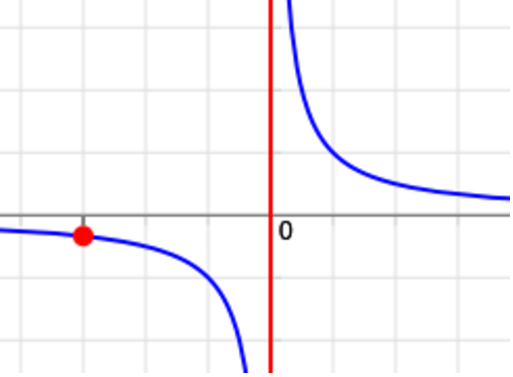
\includegraphics[width=0.3\linewidth]{images/linksseitiger_limes}
\caption{Bsp. Linksseitiger Grenzwert}
\end{figure}


\subsubsection{Rechtsseitiger Grenzwert}
Rechsseitige Grenzwerte sind Grenzwerte der Form $\lim\limits_{x \rightarrow x_0^+ }f(x)$
Man möchte dabei herausfinden wie sich die Funktion auf der Rechten Seite von $x_0$ verhält.

\subsubsection{Beidseitiger Grenzwert}
Der (beidseitige) Grenzwert $\lim\limits_{x \rightarrow x_0} f(x)$ existiert nur, wenn gilt:

$\lim\limits_{x \rightarrow x_0^- }f(x)$ = $\lim\limits_{x \rightarrow x_0^+ }f(x)$


\subsubsection{Grenzwerte bei stetigen Funktionen}
Der Grenzwert einer stetigen Funktion an der Stelle $x_0$ entspricht dem Funktionswert an dieser Stelle, sofern $x_0$ zur Definitionsmenge der Funktion gehört.
\begin{align*}
\lim\limits_{x \rightarrow x_0} f(x) = f(x_0)
\end{align*}

\subsubsection{Der Regel von Bernoulli und L'Hospital}
Gibt es Grenzwerte vom einem der folgenden Typen, können die beiden Funktion abgeleitet und von der Ableitung der Grenzwert bestimmt werden.
\begin{itemize}
	\item Typ $ \frac{\lim\limits_{x \rightarrow a}{f(x)}}{\lim\limits_{x \rightarrow a}{g(x)}} =  \frac{0}{0}$
	\item Typ $\frac{\lim\limits_{x \rightarrow a}{f(x)}}{\lim\limits_{x \rightarrow a}{g(x)}} = \frac{\infty}{\infty}$
	\item dann $\lim\limits_{x \rightarrow a}{\frac{f(x)}{g(x)}} = \lim\limits_{x \rightarrow a}{\frac{f'(x)}{g'(x)}}$
\end{itemize}


\subsubsection{Vorgehen}
\begin{enumerate}
\item Ausdruck so weit wie möglich vereinfachen. Falls mit einem direkten Einsetzen kein Arithmetischer Fehler (z.B Teilen durch Null) provoziert wird, kann man den Grenzwert direkt für $x$ einsetzen.
\item Endlicher Grenzwert für $x$ einsetzen
\item Grenzwert berechnen	
\end{enumerate}



\section{Integration}

\subsection{Stammfunktion}
Man nennt eine Funktion $F(x)$ Stammfunktion von $f(x)$, wenn die Ableitung der Stammfunktion $f(x)$ ergibt. 
\[F'(x) = f(x)\]

\subsubsection{Vorgehen}
Generell versucht man immer die Funktion zu finden, die abgeleitet den gegebenen Term ergibt. Besonders einfach gestaltet sich die Suche für Terme mit Exponenten. Dabei erhöht man den gegebenen Exponenten um 1 und kompensiert mit $\frac{1}{\text{Exponent + 1}}$
\paragraph{Beispiel}
\begin{align*}
	g(t) = \frac{1}{t^2} \Rightarrow \frac{1}{-1} \cdot \frac{1}{t^{-1}} = -t^{-1} = -\frac{1}{t} + const
\end{align*}
Von einem längere Term kann die Stammfunktion komponentenweise berechnet werden.

\subsection{Stammfunktion zeichnen}
\begin{enumerate}
	\item Startwert ist der Wert ganz links vom Intervall
	\begin{itemize}
		\item Falls die Stammfunktion an einer bestimmten Stelle gesucht ist muss der finale Graph noch an der Ordinate verschoben werden.
	\end{itemize}
	\item Für jedes Teil-Intervall die Punkte für die Stammfunktion einzeichnen: Fläche = x-Wert ganz Rechts vom Intervall
	\item Steigung einzeichen: Falls der Graph im Intervall eine konstante Steigung hat, ist der Graph der Stammfunktion linear. Ansonsten ist der Graph gemäss der Funktion der Stammfunktion (Parabel, Sinus, etc.)
\end{enumerate}

\subsection{Unbestimmtes Integral}
\begin{itemize}
	\item Das unbestimmte Integral repräsentiert eine Menge von Stammfunktionen
\end{itemize}
\subsubsection{Definition}
\[
\int \underbrace{f(x)}_{{\text{Integrand}}}\, \underbrace{dx}^{{\text{Integrationsvariable}}} = F(x) + \underbrace{\text{ const}}_{{\text{Integrationskonstante}}}
\]

ist $\Leftrightarrow$ zu:

\[
f(x) = \frac{d}{dx}(F(x + \text{ const}))
\]

\subsubsection{Linearitätsregel}
\begin{align}
\int c \cdot f(x) + c \cdot g(x) \cdot dx &= c\int f(x) \cdot dx + c \int g(x) \cdot dx
\end{align}
\subsubsection{Substitutionsregel}
\paragraph{Vorraussetzungen}
\begin{itemize}
	\item Integrant muss ein Produkt sein und ein Faktor muss verschachtelt sein
	\item Der andere Faktor muss die Ableitung der inneren Komponente der Verschachtelung sein.
\end{itemize}
\[
\int f(g(x)) \cdot g'(x) dx = F(g(x)) + const
\]

\paragraph{Vorgehen}
Beispiel: $\int cos(ln(x)) \cdot \frac{1}{x} dx$

\begin{enumerate}
	\item Innere Komponente der Verschachtelung mit der Variablen u ersetzen
	\item Stammfunktion der äusseren Komponente der Verschachtelung suchen: $\int \cos(u) du = \sin(u) \text{+ const}$
	\item Falls Stammfunktion bei Punkt 2. vorhanden, Rücksubstitution von u: = \underline{\underline{$\sin(\ln(x)) + const $}}
\end{enumerate}

\subsubsection{Partielle Integration}
\paragraph{Voraussetzungen}
\begin{itemize}
	\item Der Integrant besteht aus zwei Faktoren
	\item Sei die erste Funktion f(x) eine Funktion mit bekannter Stammfunktion F(x) die zweite Funktion g(x) irgendeine ableitbare Funktion, dann kann mit folgender Gleichung gearbeitet werden.
\end{itemize}
\begin{align}
	\int f(x)\cdot g(x) dx = \underbrace{F(x)}_{Stammfunktion} \cdot \underbrace{g(x)}_{Ableitbare Funktion} - \int \underbrace{F(x)}_{Stammfunktion}\cdot \underbrace{g'(x)}_{Ableitung}dx
\end{align}

\subsubsection{Spezialfälle}
Folgende Spezialfälle Funktionieren immer dann wenn ein Faktor die Ableitung des jeweilig anderen ist.
\[
\int f(ax + b) dx = \frac{1}{a} F(ax + b) + const
\]
\[
\int f(x) \cdot f'(x) dx = \frac{1}{2} f(x)^2 + const
\]
\[
\int f^q(x) \cdot f'(x) dx = \frac{1}{q+1} f^{q+1} (x) + const
\]
\[
\int \frac{f'(x)}{f(x)} dx = ln(|f(x)|) + const
\]


\paragraph{Vorgehen}
\begin{enumerate}
	\item Eine Funktion ableiten und von der anderen die Stammfunktion suchen
	\item Das Integral im Resultat aus Schritt 1. auflösen
	\item Vereinfachen
\end{enumerate}

\paragraph{Beispiel}
\begin{enumerate}
	\item $\int \sin(x) \cdot x dx$
	\subitem Stammfunktion von $f(x) = F(x) = -\cos(x)$
	\subitem Ableitung von $g(x) = g'(x) = 1$
	\item 
	\begin{align*}
	\int \sin(x) \cdot x dx &= -\cos(x) \cdot x - \int -\cos(x) \cdot 1 dx \\
	&= \underline{\underline{-\cos(x) \cot x + sin(x) + const}}
	\end{align*}

\end{enumerate}

\subsection{Bestimmtes Integral}
\subsubsection{Voraussetzungen}
\begin{itemize}
	\item Das bestimmte Integral repräsentiert eine Zahl
	\item Der Integrant muss auf dem Intervall [a;b] definiert sein
	\item Ist die obere Grenze kleiner als die untere Grenze ist die Fläche negativ
	\item Es muss eine Stammfunktion von f(x) existieren
	\item $\int_{a}^{b} f(x) dx = F(b) - F(a) =
	\lim_{n \to \infty} \sum_{k=1}^{n}f(x_k) \cdot \Delta x$
\end{itemize}

\subsubsection{Flächenberechnung}
Bei der graphischen Interpretation eines Integrals $\int_{a}^{b}f(x)dx$ gibt es zwei Fälle:x
\begin{itemize}
	\item Wenn $a < b$: der Graph im positiven Bereich zählt positiv, der Graph im negativen Bereich zählt negativ.
	\item Wenn $a > b$: der Graph im positiven Bereich zählt negativ, der Graph im negativen Bereich zählt positiv.
\end{itemize}
Wird mit dem Integral die Fläche berechnet muss das Integral von dem Betrag von f(x) gerechnet werden. $\int_{a}^{b}\vert f(x) \vert$dx

\subsubsection{Rechenregeln}
\begin{itemize}
	\item Faktorregel: Konstante Faktoren dürfen aus dem Integranten herausgezogen werden $\int_{a}^{b}c \cdot f = c \cdot \int_{a}^{b}f$
	
	\item Vertauschen der Integralgrenzen ändert das Vorzeichen des Integrals:
	$\int_{a}^{b}f = - \int_{b}^{a}f$
	\item Zusammenhängende Integrale können zusammengefasst werden:
	$\int_{a}^{b}f + \int_{b}^{c}f = \int_{a}^{c}f$
	\item Linearität: $\int_{a}^{b}(f+g) = \int_{a}^{b}f + \int_{a}^{b}g$
	\item Gleiche Integrationsgrenzen $\int_{a}^{a} f = 0$
\end{itemize}

\paragraph{Bestimmtes Integral mit Betrag} \hfill \\
Beim Rechnen mit Betrag wird der Integral-Intervall in einen positiven und negativen Bereich unterteilt und dann partiell gelöst.
\begin{align}
\begin{split}
\int_{-2}^{2} |x^3| dx &= \int_{-2}^{0} -x^3 dx + \int_{0}^{2} x^3 dx \\
&= \left[\frac{1}{4}x^4 \right]_{-2}^{0} + \left[\frac{1}{4}x^4 \right]_{0}^{2} \\
&= -(0 - \frac{1}{4} (-2)^4) + (\frac{1}{4}2^4 - 0) \\
&= 4 + 4 = 8 
\end{split}
\end{align}

\subsubsection{Integralfunktion}
\[ \phi_a(x) = \int_a^x f \]
\begin{itemize}
	\item Die Integralfunktion hängt vom Parameter $a$ ab.
	\item Ändert man den Parameter $a$, so ändert sich die
	Integralfunktion nur um eine Konstante ($\phi_b(x) = \phi_a(x) + c$),
	was eine Verschiebung auf der Y-Achse bewirkt.
\end{itemize}

\subsubsection{Hauptsatz}
Jede Integralfunktion ist eine Stammfunktion. Umgekehrt kann jede
Stammfunktion zum berechnen von Integralen benutzt werden.
\[\phi_a(b) = \int_a^b f(x)dx = [F(x)]^b_a = F(b) - F(a) \]

\subsubsection{Partielle Integration}
\paragraph{Voraussetzungen}
\begin{itemize}
	\item Der Integrant besteht aus zwei Faktoren
	\item Sei die erste Funktion f(x) eine Funktion mit bekannter Stammfunktion F(x) die zweite Funktion g(x) irgendeine ableitbare Funktion, dann kann mit folgender Gleichung gearbeitet werden.
	\[
	\int\limits_{a}^{b} f(x)g(x) dx = 
	\left[ \underbrace{F(x)}_{Stammfunktion} \cdot \underbrace{g(x)}_{Ableitbare Funktion} \right] _a^b
	- \int\limits_{a}^{b} \underbrace{F(x)}_{Stammfunktion} \cdot \underbrace{g'(x)}_{Ableitung}dx
	\]
\end{itemize}
\paragraph{Vorgehen}
\begin{enumerate}
	\item Eine Funktion ableiten und von der anderen die Stammfunktion suchen
	\item Das Integral im Resultat aus Schritt 1. auflösen
	\item Vereinfachen
\end{enumerate}

\subsubsection{Spezialfälle}
Folgende Spezialfälle Funktionieren immer dann wenn ein Faktor die Ableitung des jeweilig anderen ist.
\[
	\int_{a}^{b} f(ax + b) dx = \left[ \frac{1}{a} F(ax + b) \right]_{a}^{b}
\]
\[
\int_{a}^{b} f(x) \cdot f'(x) dx = \left[\frac{1}{2} f(x)^2 \right]_{a}^{b}
\]
\[
\int_{a}^{b} f^q(x) \cdot f'(x) dx = \left[\frac{1}{q+1} f^{q+1} (x) \right]_{a}^{b} 
\]
\[
\int_{a}^{b} \frac{f'(x)}{f(x)} dx = \left[ln(|f(x)|) \right]_{a}^{b}
\]

\subsubsection{Substitutionsregel}
\paragraph{Vorraussetzungen}
\begin{itemize}
	\item Integrant muss ein Produkt sein und ein Faktor muss verschachtelt sein
	\item Der andere Faktor muss die Ableitung der inneren Komponente der Verschachtelung sein.
\end{itemize}
\begin{align}
\begin{split}
	 \int_a^b f(g(x)) \cdot g'(x) dx &= \int_{g(a)}^{g(b)} f(u) du \\
	 &= \left[ F(u) \right]_{g(a)}^{g(b)} \\
	 &= F(g(b)) - F(g(a))
\end{split}
\end{align}

\paragraph{Vorgehen}
Beispiel: $\int_{0}^{\pi} (e^{-cos(x)} \cdot sind(x ) dx$

\begin{enumerate}
	\item Innere Komponente der Verschachtelung mit der Variablen u ersetzen und neue Intervalsgrenzen definieren
	\item Stammfunktion der äusseren Komponente der Verschachtelung suchen: $\int_{-cos(0)}^{-cos(\pi)} e^u du $
	\item Falls Stammfunktion bei Punkt 2. vorhanden, Rücksubstitution von u: = $\left[e^u\right]_{-1}^{1} = e - e^-1$
\end{enumerate}

	
\section{Fourierreihen}
Eine Fourierreihe der Funktion s(t) besteht aus einer Linearkombination
von Sinus- und Kosinus-Funktionen, welche alle dieselbe Persiode $T$
haben. Je höher die Ordnung n, desto genauer wird die ursprüngliche Funktion s(t) aproximiert.

\paragraph{Periode bestimmen}
\[
	\text{Periode T von } sin(yx) = \frac{2\pi}{y}
\]

\subsection{Sinus-Kosinus-Form}
\[
f(t) = a_0 + \sum_{k=1}^{n}
(a_k \cdot \cos(k \omega_1 t) + b_k \cdot \sin(k \omega_1 t))
\]
\begin{itemize}
	\item Periode $T$
	\item Grundkreisfrequenz $\omega_1 = \frac{2\pi}{T}$
	\item Signalmittelwert $a_0 =  \frac{1}{T}\int_0^T s(t) dt$
	\item Koeffizient $a_k = \frac{2}{T} \int_0^T s(t) \cdot \cos(k \omega_1 t) dt$
	\item Koeffizient $b_k = \frac{2}{T} \int_0^T s(t) \cdot \sin(k \omega_1 t) dt$
\end{itemize}

\subsection{Amplituden-Phasen-Form}
\[
f(t) = A_0 + \sum_{k=1}^{n}
(A_k \cdot \cos(k \omega_1 t  - \varphi_k))
\]
\begin{itemize}
	\item Periode $T$
	\item Grundkreisfrequenz $\omega_1 = \frac{2\pi}{T}$
	\item Konstante $A_0 = a_0$
	\item Koeffizient $A_k = \sqrt{a_k^2 + b_k^2}$
	\item $\varphi_k =  \begin{cases}
	arctan\left(\frac{b_k}{a_k}\right) & \text{ für } a_k > 0 \\
	arctan\left(\frac{b_k}{a_k}\right) + \pi & \text{ für } a_k < 0 \\
	\frac{\pi}{2} & \text{ für } a_k = 0 \wedge b_k > 0\\
	-\frac{\pi}{2} & \text{ für } a_k = 0 \wedge b_k < 0\\
	\end{cases}$
\end{itemize}

\subsection{Vorgehen}
\begin{enumerate}
	\item Grundperiode T beim gegebenen Signal s(t) herauslesen
	\item Grundkreisfrequenz berechnen $\omega_1 = \frac{2\pi}{T}$
	\item Falls s(t) gerade oder ungerade, fällt ein Koeffizient automatisch weg. 
	\item $a_0$ bestimmen: Falls $a_k = 0$ ist auch $a_0 = 0$ 
	\begin{enumerate}
		\item Partielle Integration: Grundperiode in Bereiche aufteilen, sodass für jeden Bereich der Funktionswert von s(t) bestimmt werden kann. 
		\item s(t) mit Funktionswert ersetzen
	\end{enumerate}
	\item $a_0$ bestimmen:
	\begin{enumerate}
		\item $a_0 =  \begin{cases}
		0 & \text{ für s(t) ungerade (punktsymmetrisch am Nullpunkt)} \\
		\frac{2}{T} \cdot \int_{0}^{\frac{T}{2}} s(t) dt & \text{ für s(t) gerade (spiegelsymmetrisch an der Y-Achse)} \\
		\end{cases}$
	\end{enumerate}
	\item $a_k$ bestimmen:
	\begin{enumerate}
		\item $a_k =  \begin{cases}
		0 & \text{ für s(t) ungerade (punktsymmetrisch am Nullpunkt)} \\
		\frac{4}{T} \cdot \int_{0}^{\frac{T}{2}} s(t) \cdot \cos(k \omega_1 t) dt & \text{ für s(t) gerade (spiegelsymmetrisch an der Y-Achse)} \\
		\end{cases}$
	\end{enumerate}
	\item $b_k$ bestimmen:
	\begin{enumerate}
		\item $b_k =  \begin{cases}
		0 & \text{ für s(t) gerade (spiegelsymmetrisch an der Y-Achse)} \\
		\frac{4}{T} \cdot \int_{0}^{\frac{T}{2}} s(t) \cdot \sin(k \omega_1 t) dt & \text{ für s(t) ungerade (punktsymmetrisch am Nullpunkt)}  \\
		\end{cases}$
		\item Weiter muss mittels partieller Integration die Integrale aufgelöst wer
		\item Von der trigonometrischen Funktion prüfen wie viele Lösungen die trigonometrische Funktion zurückgeben kann (In Abhängigkeit von k). (z.B Bei einem Funktionsargument von $\frac{k\pi}{2} \Rightarrow k= 4 \Rightarrow 360^\circ$ Lösungen)
		\item Die einzelnen Lösungen notieren
	\end{enumerate}
	\item $a_0, a_k, b_k$ in Fourierformel einsetzen 
	\item Für jedes k die Summe aufschreiben	
\end{enumerate}


\subsection{Umformungen}
\subsubsection{Sinus Cosinus Form $\Rightarrow$ Amplituden Phasen Form}
\paragraph{Grafisch}
\begin{figure}[h]
	\centering
	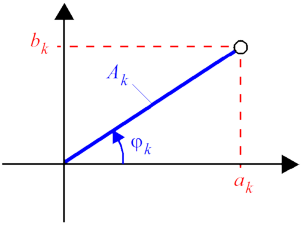
\includegraphics[width=0.3\linewidth]{images/sincos_ampform_transformation}
	\caption{Umformung}
\end{figure}
Man rechnet die kartesischen der Sinus Cosinus Form )($a_k, b_k$) in die polaren Koordinaten der Amplituden Phasen Form ($A_k, \varphi_k$) um.

\[A_k = \sqrt{a_k^2 + b_k^2}\]

Für $\varphi_k$ sind verschiedene Fälle zu beachten:

\begin{enumerate}
	\item Wenn der Punkt in der rechten Halbebene liegt, so gilt:
	\[\varphi_k = arctan(\frac{b_k}{a_k})\]
	\item Wenn der Punkt in der linken Halbebene liegt so gilt:
	\[\varphi_k = arctan(\frac{b_k}{a_k}) + \pi \]
	\item Wenn der Punkt auf der Ordinatenachse liegt (Y-Achse) dann ist der Richtungswinkel entweder:
	\begin{itemize}
		\item obere Halbachse = $\frac{\pi}{2}$
		\item untere Halbachse = $-\frac{\pi}{2}$
	\end{itemize}
	\item Wenn der Punkt auf dem Ursprung liegt gibt es kein $\varphi_k$
\end{enumerate}

\paragraph{Quadrantenbeziehungen}
Ist s(t) ungerade oder gerade können die Koeffizienten $a_k$ und $b_k$ sowie die Funktionsargumente der trigonometrischen Funktionen mit den Quadrantenbeziehungen 1:1 umgeformt werden.
\[
\cos(x - \frac{\pi}{2}) = \sin(x)
\]
\[
\cos(x - \pi) = -\cos(x)
\]
\[
\cos(x - \frac{3\pi}{2}) = -\sin(x)
\]
\[
\cos(x - 0) = \cos(x)
\]

\subsubsection{Amplituden Phasen Form $\Rightarrow$ Sinus Cosinus Form}
\paragraph{Grafisch}
Man rechnet die polaren Koordinaten der Amplituden Phasen Form ($A_k, \varphi_k$)in die kartesischen der Sinus Cosinus Form )($a_k, b_k$) um. 

\[ a_k = A_k \cdot cos(\varphi_k) \]
\[ b_k = A_k \cdot sin(\varphi_k) \]

\paragraph{Hinweis}
Je nach Situation kann man auch versuchen die gegebenen cos(x) Terme mit den Additionstheoremen umzuwandeln.

\begin{figure}[h]
\centering
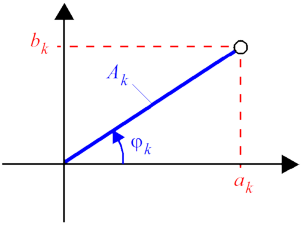
\includegraphics[width=0.3\linewidth]{images/sincos_ampform_transformation}
\caption{Umformung}
\end{figure}

\section{Vergleiche}
\subsection{Taylorreihe und Fourierreihe}
\begin{tabu} to \linewidth {|X|X|X|}
	\hline
	& Taylorreihe & Fourierreihe \\ 
	\hline
	Input & Funkktion, die sich of Ableiten lässt. Entwicklungspunkt $x_0$ & periodische Funktion \\ \hline
	Bausteine & Polynome $(x - x_0)^k;k\in \mathbb{N}$ & sin(kx) und cos(kx) Terme; $k \in \mathbb{N}$\\ \hline
	Approximatives Verhalten & Vom Entwicklungspunkt weg von innen nach aussen & global (von groben zu feinen Strukturen) \\ \hline
	Berechnung der Koeffizienten & Durch Ableiten an Enwiclungspunkt & Durch Minimieren der Fehlerfläche \\ \hline
\end{tabu}

\end{document}